\documentclass[12pt, a4paper]{article}
\usepackage[spanish,es-tabla]{babel}
\usepackage[utf8]{inputenc}
\usepackage[T1]{fontenc}
\usepackage{lmodern}
\usepackage{graphicx}
\usepackage{amsmath}

\makeatletter
\newcommand\setItemnumber[1]{\setcounter{enum\romannumeral\@enumdepth}{\numexpr#1-1\relax}}
\makeatother

\title{Arquitectura de Microprocesadores}
\author{Gianfranco Talocchino}
\date{Marzo - Abril de 2022}

\begin{document}
\maketitle

\section{Preguntas orientadoras}
\subsection{Introducción}
\begin{enumerate}
    \item Describa brevemente los diferentes perfiles de familias de 
    microprocesadores/microcontroladores de ARM. Explique alguna de sus 
    diferencias características.
    
    La familia de arquitecturas ARM Cortex esta dividida en tres 
    principales subfamilias.
    
    \begin{itemize}
        \item Cortex A (\emph{\textbf{A}pplication}): Es la que ofrece mayor rendimiento. Está 
        orientada la ejecución de sistemas operativos como \emph{Linux} y derivados. Su 
        aplicación principal son computadoras, celulares, \emph{tablets}, etc.
        \item Cortex R (\emph{\textbf{R}eal-Time}): Esta orientada y optimizada a aplicaciones 
        \emph{real-time}. Su aplicación se centra en la industria médica, aeronáutica, etc.
        \item Cortex M (\emph{\textbf{M}icrocontrollers}): Esta orientada al uso en 
        microcontroladores y sistemas embebidos de propósito general.
    \end{itemize}
\end{enumerate}
\subsection{Cortex M}
\begin{enumerate}
    \item Describa brevemente las diferencias entre las familias de procesadores Cortex M0, M3 
    y M4.
    
    A grandes rasgos la diferencia es el costo, la velocidad y el consumo de energía. Los 
    Cortex M0 están optimizados para ocupar la menor cantidad de silicio y ser lo mas baratos 
    posible. Frente a los Cortex M3 las diferencias a nivel de Hardware se traducen en
    que algunos core peripherals son opcionales, una arquitectura de memoria Von Neumann y la 
    falta de MPU. Por otro lado, los Cortex M4 añaden la posibilidad de contar opcionalmente 
    con una FPU e instrucciones de DSP. De esta manera, entre los Cortex M0 y M4 el rendimiento
    es creciente, asi como también el costo y el consumo de energía debido a la mayor cantidad 
    de features implementadas en hardware.
    
    \item ¿Por qué se dice que el set de instrucciones Thumb permite mayor densidad de código?
    Explique.
    
    El set de instrucciones Thumb permite mezclar instrucciones de 16 y 32 bits sin que exista una 
    sobrecarga asociada al cambio. Esto da lugar a que operaciones mas simples puedan ser llevadas 
    a cabo con instrucciones de 16 bits en vez de 32 bits. Como resultado, se logra 
    una mayor densidad de código que al solo utilizar instrucciones de 32 bits para operaciones 
    simples y complejas.
        
    \item ¿Qué entiende por arquitectura load-store? ¿Qué tipo de instrucciones no posee este
    tipo de arquitectura?
    
    Una arquitectura de hardware load-store es aquella que solo las instrucciones load y store 
    acceden a memoria RAM. El resto de operaciones (aritméticas, lógicas, etc ..) usan solo 
    registros internos del procesador.
    
    \item ¿Cómo es el mapa de memoria de la familia?
    Los Cortex M tiene un sistema de memoria con direcciones de 32 bits que
    generan un espacio de lineal de direcciones de 4GB. El cual, está participando en 
    número de regiones asignados a diferentes usos. En la Figura \ref{fig:map} se muestra
    un ejemplo.
    \begin{itemize}
        \item Código de programa
        \item RAM
        \item Periféricos
        \item Registros de control
    \end{itemize}
    
    \begin{figure}[!ht]
        \centering
        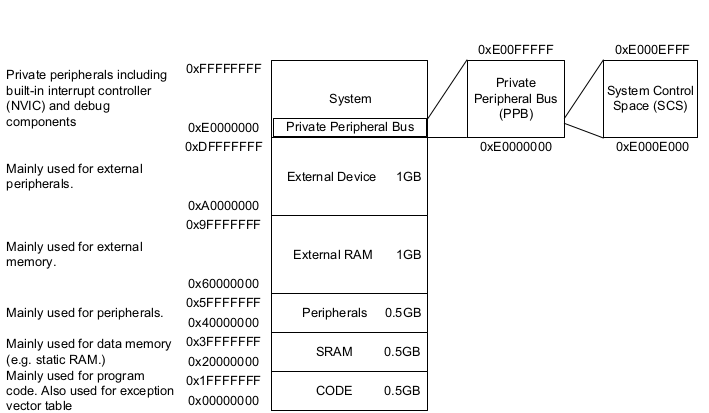
\includegraphics[scale=0.6]{map}
        \caption{Mapa de memoria de la familia Cortex M.}
        \label{fig:map}
    \end{figure}
    
    \item ¿Qué ventajas presenta el uso de los “shadowed pointers” del PSP y el MSP?
    
    ARM Cortex M tiene dos stack pointers. Se encuentran en diferentes bancos por lo 
    tanto solo uno es visible en un momento dado. Los dos stack pointers son los siguientes
    \begin{itemize}
        \item Main Stack Pointer (MSP)
        \item Process Stack Pointer (PSP)
    \end{itemize}
    
    El MSP generalmente es reservado para el uso del kernel y manejos de excepciones mientras que 
    PSP se utiliza en las tareas. La ventaja que presenta es que el MSP se encuentra protegido del
    stack del usuario incluso si el stack de usuario hizo overflow. Esto facilita la implementación
    de sistemas operativos.
    
    \item Describa los diferentes modos de privilegio y operación del Cortex M, sus relaciones y 
    como se conmuta de uno al otro. Describa un ejemplo en el que se pasa del modo 
    privilegiado a no privilegiado y nuevamente a privilegiado.
  
    Los modos de operación del Cortex M son:
    \begin{itemize}
        \item Thumb: Modo cuando el procesador está corriendo código de programa.
        \item Debug: Modo cuando el procesador detuvo la ejecución de instrucciones
    \end{itemize}
    
    Los modos de privilegio son:
    
      \begin{itemize}
        \item Unprivileged: El procesador ejecuta código que tiene restricciones como por ejemplo
        el acceso a ciertas áreas de memoria y ciertos registros de control
        \item Privileged: El es estado por defecto donde el procesador ejecuta código sin restricciones de 
        acceso.
    \end{itemize}
    
    Los modos de acceso son:
    
    \begin{itemize}
        \item Handler: El procesador esta ejecutando el handler de una excepción. Siempre
        lo hace en modo privilegiado.
        \item Thread: El procesador ejecuta código de aplicación. Puede ser en modo 
        privilegiado y no privilegiado.
    \end{itemize}
    
    De modo privilegiado a no privilegiado se puede pasar simplemente seteando el registro CONTROL en el bit 0.
    Para pasar de modo no privilegiado a privilegiado es necesario generar una excepción y borrar el bit 0 
    del registro CONTROL.

    \setItemnumber{7}
    \item ¿Qué se entiende por modelo de registros ortogonal? Dé un ejemplo
    
    Se dice que una arquitectura de hardware posee un modelo de registros ortogonales 
    cuando el conjunto de instrucciones no impone la limitación de que una cierta instrucción
    deba utilizar exclusivamente un registro especifico. La arquitectura ARM Cortex M posee
    modelo de registros ortogonales. Otras arquitecturas como x86 no.
    
    
    \setItemnumber{8}
    \item ¿Qué ventajas presenta el uso de instrucciones de ejecución condicional (IT)? Dé un
    ejemplo
    
    El uso de instrucciones de ejecución condicional reduce el numero de instrucciones de salto
    en un programa. Esto por un lado mejora la densidad de código y por otro aumenta el rendimiento.
    Por ejemplo, las instrucciones de salto con costosas para el procesador ya que toma tres ciclos de 
    reloj rellenar nuevamente el pipeline luego de un salto. 

    \setItemnumber{9}
    \item Describa brevemente las excepciones más prioritarias (reset, NMI, Hardfault).
    
    \begin{description}
        \item [Reset:] Esta excepcion es lanzada justo despues de que el procesador se reinicia.
        Su manejador es realmente el punto de entrada del programa que se esta ejecutando.
        \item[NMI:] se trata de una excepción especial, que tiene la máxima prioridad después de 
        la de reset. Al igual que la excepción de reset, no puede ser enmascarada (es decir, desactivada), 
        y puede ser asociada a actividades críticas e inaplazables.
        \item[Hardfault:] es la excepción de fallo genérica, y por tanto relacionada con las excepciones de 
        software. Cuando las otras excepciones están deshabilitadas, actúa como colector de todo tipo de 
        excepciones (por ejemplo, un acceso a la memoria a una ubicación no válida, se activan las 
        excepciones de hard fault si la de bus fault no está activada).
        
    \end{description}
    
    \setItemnumber{10} 
    \item Describa las funciones principales de la pila. ¿Cómo resuelve la arquitectura el llamado 
    a funciones y su retorno?
    
    Las funciones principales de la pila son:
    
    \begin{itemize}
        \item Cuando un programa ejecuta una función que utiliza los registros internos del procesador, 
        los datos que contienen estos registros son almacenados temporalmente en el stack para luego ser
        restaurados al final de la ejecución de la función.
        \item Para almacenar del estado del procesador y los valores de los registros internos en 
        el caso de que ocurra una excepción.
        \item Para almacenar variables locales.
        \item Para el pasaje de los parámetros de funciones en C que son llamadas siguiendo 
        el "Procedure Call Standard". En este caso recién a partir del quinto parámetro se 
        comienzan a almacenar en el stack.
     \end{itemize}
    
    \setItemnumber{11} 
    \item Describa la secuencia de reset del microprocesador.
    
    Tras el reinicio y antes de que el procesador comience a ejecutar el programa, los procesadores 
    Cortex M leen las dos primeras palabras de la memoria. El principio del espacio de memoria contiene
    la tabla de vectores, y las dos primeras palabras de la tabla de vectores son el valor inicial para el 
    Main Stack Pointer (MSP). vector son el valor inicial del puntero de la pila principal (MSP), 
    y el vector de reset, que es la dirección inicial del reset handler. Después de que el procesador 
    lea estas dos palabras, el procesador configura el MSP y el contador de programa (PC) con estos 
    valores.
    
    
    \setItemnumber{12}
    \item ¿Qué entiende por ``core peripherals''? ¿Qué diferencia existe entre estos y 
    el resto de los periféricos?
    
    Se entiende por ``core peripherals'' a aquellos periféricos que son específicos del 
    procesador, en este caso, procesadores de la familia Cortex M. Se diferencian de los 
    periféricos añadidos por los fabricantes de microcontroladores en que estos son provistos 
    por ARM. El resto, si bien puede agregar las mismas funcionalidades su implementación y capacidad
    variarán notablemente entre fabricantes. Algunos ejemplos de core peripherals para ARM Cortex M 
    incluyen el NVIC, el SysTick, la MPU.
    
    \setItemnumber{14}
    \item ¿Qué es el CMSIS? ¿Qué función cumple? ¿Quién lo provee? ¿Qué ventajas aporta?
    
    El estándar llamado Common Microcontroller Software Interface Standard (CMSIS) desarrollado por 
    ARM es un capa de abstracción para microcontroladores Cortex M. Se encargar de definir interfaces
    para acceso al hardware genérico que estos comparten. Entre las ventajas que aporta se encuentran:
    
    \begin{itemize}
        \item Reduce la curva de aprendizaje del programador.
        \item Reduce los costos de desarrollo.
    \end{itemize}
    
    \setItemnumber{16}
    \item Explique las características avanzadas de atención a interrupciones: tail chaining y late
    arrival.
    
    \begin{itemize}
        \item tail chaining: Es una optimización realizada en el manejo de interrupciones en donde 
        interrupciones consecutivas se atienden sin la necesidad de guardar y restaurar el contexto del 
        procesador nuevamente  
        
        \item late arrival: Es una característica en la cual si una interrupción con mayor prioridad 
        llega mientras atiende una de menor prioridad, el Cortex-M detiene el proceso y atiende primero 
        la interrupción de mayor prioridad.
    \end{itemize}
    
    
    \setItemnumber{17}
    \item ¿Qué es el systick? ¿Por qué puede afirmarse que su implementación favorece la portabilidad 
    de los sistemas operativos embebidos?
    
    Systick es simplemente un timer presente dentro los microcontroladores basados en ARM Cortex M. 
    En sistemas operativos de tiempo real se usa como temporizador del planificador de tareas. Al 
    estar definido por ARM y no variar de un fabricante de microcontrolador a otro facilita
    su portabilidad. Esto ocurre ya que no se necesita cambiar esta fuente de temporización 
    constantemente cuando se pasa de un microcontrolador a otro.
    
    \setItemnumber{18}
    \item ¿Qué funciones cumple la unidad de protección de memoria (MPU)?
    
    El principal propósito de una unidad de protección de memoria (MPU) es proteger regiones de
    memoria definiendo diferentes permisos de accesos a estas. Estos permisos dependerán de un 
    nivel de privilegio y facilitan la implementación de sistemas operativos.
    
    \setItemnumber{19}
    \item¿Cuántas regiones pueden configurarse como máximo? ¿Qué ocurre en caso de haber solapamientos de 
    las regiones? ¿Qué ocurre con las zonas de memoria no cubiertas por las regiones definidas?
    
    La unidad de protección de memoria en los Cortex M3 y M4 permite hasta un máximo de 8 regiones 
    programables de memoria. Cuando se producen solapamientos los permisos y atributos de esa región de 
    memoria serán los que correspondan a la región de numeración mas alta. El acceso  a zonas de memoria 
    no cubiertas por las regiones definidas disparará excepciones del tipo Memory Management Fault si 
    la excepción está activada o por defecto si no esta activa disparará una excpeción de tipo Hard Fault.
    
\end{enumerate}

\subsection{ISA}

\begin{enumerate}
    \item ¿Qué son los sufijos y para qué se los utiliza? Dé un ejemplo
    
    Los sufijos son modificadores que pueden agregarse opcionalmente a algunas instrucciones. Se 
    colocan al final del mnemónico.
    
    Existen tres tipos de sufijo en assembler para ARM Cortex M
    
    \begin{itemize}
        \item Sufijo "s": permite indicar opcionalmente si instrucciones actualizan el 
        Application Program Status Register (APSR).
        \item Sufijo de ejecución condicional: permiten ejecutar instrucciones.
        condicionalmente
        \item Sufijos de precisión: permiten indicar la cantidad de bits involucrados en la operación
        de una instrucción. Para Cortex M existen 3 tipos:
        \begin{itemize}
            \item byte (b): 8 bits
            \item halfword (h): 16 bits
            \item word (w): 32 bits
        \end{itemize}
    \end{itemize}

    \item ¿Para qué se utiliza el sufijo ‘s’? Dé un ejemplo
    
    El sufijo "s" se utiliza para que durante la ejecución de una instrucción se actualice 
    opcionalmente los flags del carry, overlfow, cero y negativo (Application Program Status Register)
    
    \item ¿Qué utilidad tiene la implementación de instrucciones de aritmética saturada? Dé un 
    ejemplo con operaciones con datos de 8 bits.
    
    La implementación de aritmética saturada tiene varias ventajas practicas. Permite detectar overflow 
    de sumas y multiplicaciones en forma mas consistente y simple con una sola comparación con el valor
    máximo o mínimo. Además, permite implementar algoritmos utilizados en procesamiento digital de
    señalas más eficientemente. Por ejemplo, ajustar el nivel de una señal puede resultar en un overflow
    y la saturación causa una distorsión significativamente menor que la provocada por el overlfow.
    
    A continuación se muestra un ejemplo de operación de utilizando aritmética saturada para 8 bits.
    
    \begin{equation}
    \begin{split}
    100 &+ 20 \rightarrow{} 120 \\
    100 &+ 60 \rightarrow{} 127 \,\, \text{(no -96)} \\
    100 &+ 28 \rightarrow{} -127  \,\,  \text{(no -128)} \\
    -50 &- 5 \rightarrow{} -55 \\
    -50 &- 90 \rightarrow{} -128  \,\,  \text{(no 140)} \\
    -90 &- 100 \rightarrow{} -128  \,\,  \text{(no 190)}
    \end{split}
    \end{equation}
    
    
    \item Describa brevemente la interfaz entre assembler y C ¿Cómo se reciben los argumentos de las 
    funciones? ¿Cómo se devuelve el resultado? ¿Qué registros deben guardarse en la pila 
    antes de ser modificados?
    
    El mecanismo que define la interfaz entre assembler y C se llama "Procedure Call Standard" (PCC) y 
    esta definido por ARM. En él, se especifica que los los primeros cuatro parámetros de una función 
    se pasan en los registros r0, r1, r2 y r3. El resultado debe devolverse a través del registro r0. 
    En caso de que se pasen mas de 4 parámetros el pasaje debe hacerse a través del stack. Los registros 
    restantes r4-10, pc y lr deben guardarse en el stack para ser preservados antes de utilizarse.
    
    \item¿Qué es una instrucción SIMD? ¿En qué se aplican y que ventajas reporta su uso? Dé un ejemplo.
    
    Se entiende por una instrucción SIMD (Single instruction, multiple data) a aquella que aplica en 
    paralelo la misma operación sobre un grupo de datos que comúnmente se conoce como vector.
    
    Una aplicación que puede aprovechar las ventajas de SIMD es aquella en la que el mismo valor 
    se suma a (o se resta de) un gran número de puntos de datos, una operación habitual en muchas 
    aplicaciones multimedia y de procesamiento de señales.
    
    Un ejemplo sería cambiar el brillo de una imagen. Cada píxel de una imagen consta de tres valores 
    para el brillo, los componentes rojo (R), verde (G) y azul (B) del color. Para cambiar el brillo, 
    los valores R, G y B se leen de la memoria, se les suma (o resta) un valor y los valores 
    resultantes se escriben de nuevo en la memoria.
    
\end{enumerate}

\end{document}

